\section{Introduction}
\subsection{Context}
LIFE (\textit{Large Interferometer for Exoplanets} \cite{Life1}) is a mission concept consisting of multiple free-flying telescopes operating together as a nulling interferometer in space. It is proposed to directly image the thermal emission of low-mass temperate exoplanets in the mid-infrared. The mission is split into two approximately equally long phases: a search phase and a characterization phase. The mission shares many similarities with NASA's proposed HWO (\textit{Habitable Worlds Observatory} \cite{HWO}).

Mission yield estimates for HWO and LIFE typically follow one of two approaches: Either using partially theoretical, partially empirical occurrence rates to model exoplanet yields, or using the currently known exoplanet population for such predictions \cite{Life10}. The latter may fall victim to observational biases in a stronger way, but presents the advantage of giving a potential target list for the search phase. This report builds on the latter approach.

 In previous work, \textcite{Menti_2024} with LIFEcat and \textcite{hpic} with HPIC (\textit{Habitable Worlds Observatory Preliminary Input Catalog}) have compiled catalogs of stars based on physical criteria (temperature, age, flare activity) and mission-specific requirements (magnitude in a range of bands, distance). Since the HWO and LIFE missions share many observation goals---and while LIFEcat is still in development---HPIC can be used to help with LIFE target selection. A current working version of a stellar catalog extends the HPIC catalog by adding non-binary M-dwarfs from LIFEcat to the catalog. This group of stars was discarded when compiling HPIC due to HWO's brightness requirements in near-IR to UV, but these stars may be observable with LIFE's mid-IR wavelength range. This catalog will be referred to as HPICxLIFEcat in this report.
 
 Crossmatching describes the process of identifying corresponding objects between two astronomical catalogs. This work focuses on finding the already detected planets around the HPICxLIFEcat stars, and provides a general Python package for matching a stellar catalog to a planetary catalog, outputting a combined catalog with combined columns. We take an approach that is agnostic to both the stellar catalog used, such that future iterations of a stellar target selection catalog can easily be processed, and to the planetary catalog used, such that different data sources may be swapped easily. The NASA Exoplanet Archive \cite{NasaExoplanetArchive} and Exo-MerCat \cite{Alei_2020, Alei_2025} are the catalogs this project was specifically developed for. In this project we differentiate between coordinate-based and identifier-based crossmatching and treat both.

\subsection{Catalogs}

 The NASA Exoplanet Archive (NEA) is the most widely cited repository of confirmed exoplanets and their host-star properties. We make use of its \texttt{pscomppars} table. It aggregates and merges data from multiple published scientific sources to fill in missing gaps, prioritizing parameters based on measurement precision and recency, but also computes missing quantities. A breakdown of which columns have calculated values can be seen in \cref{fig:calculated_columns}. The methods by which the calculations are performed are documented in \url{https://exoplanetarchive.ipac.caltech.edu/docs/pscp_calc.html}, which this project makes use of at a later time. The archive also holds other tables with mission-specific exoplanet candidates, and records their promotion to confirmed planets, namely the TESS Objects of Interest Catalog \cite{TessObjectsOfInterestCatalog} and the EPIC/K2 Objects of Interest Catalog \cite{K2CandidatesAndConfirmedPlanets}, which are used indirectly through Exo-MerCat.

\begin{figure}[H]
    \centering
    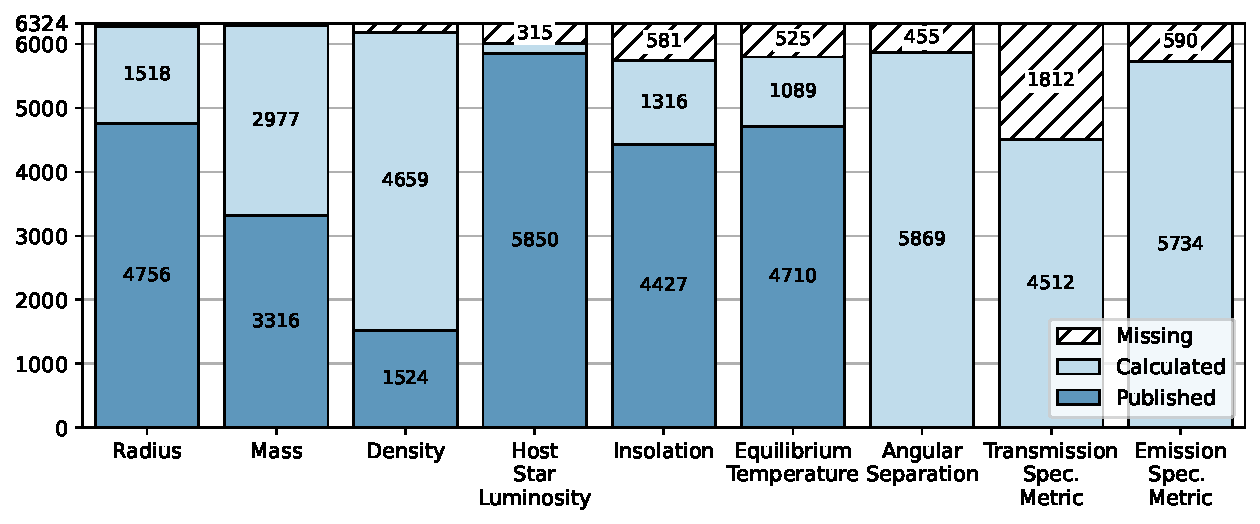
\includegraphics[width=\linewidth]{figures/nea_parameter_provenance.pdf}
    \caption{Provenance of \texttt{pscomppars} values (out of \num{6324} confirmed planets in
total) for the nine columns in which NEA reports ``Calculated Value'' entries.
All other columns are devoid of computations. Each bar splits the catalog into
entries with a directly published measurement, entries calculated by the
archive, and entries for which the parameter is missing entirely \cite{NasaExoplanetArchive}.
}
    \label{fig:calculated_columns}
\end{figure}

Exo-MerCat (\textit{Exoplanet Merged Catalog}) is a piece of Python software designed to generate a catalog of exoplanets, where data is merged from the most prominent exoplanetary catalogs (NASA Exoplanet Archive \cite{NasaExoplanetArchive}, Exoplanets Encyclopaedia \cite{ExtrasolarPlanetsEncyclopaedia}, Open Exoplanet Catalogue \cite{OpenExoplanetCatalogue}, the TESS Objects of Interest Catalog \cite{TessObjectsOfInterestCatalog} and the EPIC/K2 Objects of Interest Catalog \cite{K2CandidatesAndConfirmedPlanets}). Exo-MerCat removes computed quantities from catalogs and chooses the most precise quantities from the catalog list. 
It creates a large table with homogenized column names and units. Exo-MerCat also saves the catalogs in which it finds the planets, since a given planet may appear in multiple catalogs. A breakdown of the sources in the form of a UpSet-plot can be seen in \cref{fig:upset}. 

One important caveat that applies to both the NEA table and Exo-MerCat is that parameters for a given planet may not be self-consistent, as such planet-specific computations should be treated with caution \cite{NasaExoplanetArchive, Alei_2020, Alei_2025}. We will explicitly calculate some missing parameters. Thus all results involving some calculation, which we always clearly mark, should be treated with caution.


\begin{figure}[H]
    \centering
    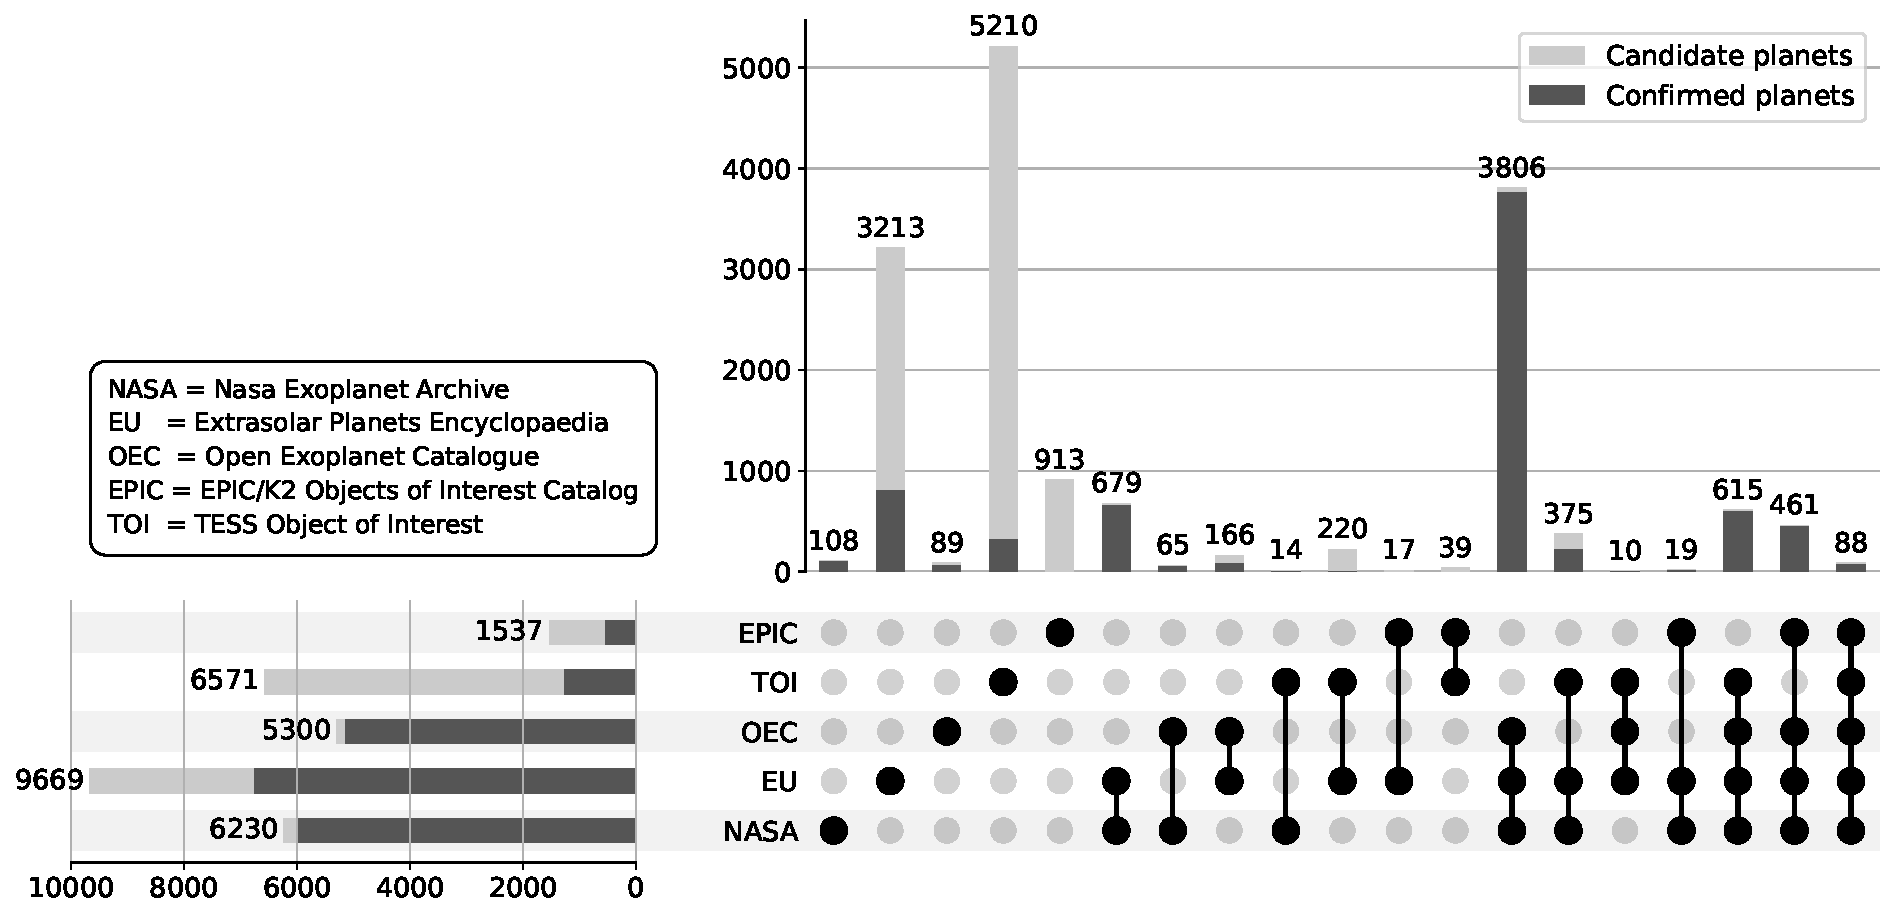
\includegraphics[width=\linewidth]{figures/exomercat_catalog_overlap_upset.pdf}
    \caption{UpSet plot showing the overlap and distribution of exoplanets across the source catalogs of Exo-MerCat. The horizontal stacked bar chart on the  left indicates the total count of planets in each catalog, while the vertical stacked bar chart at the top shows the size of the intersections of catalogs. Intersections with less than ten elements are omitted for brevity. A black dot on the line of a certain catalog means all planets in the vertical segment representing an intersection appear in that catalog. The bars are color-coded by planet status to differentiate between confirmed planets and candidate planets.}
    \label{fig:upset}
\end{figure}






\subsection{Conventions}
A candidate exoplanet is a suspected planetary signal that requires further validation to rule out astrophysical false positives. Conversely, a confirmed exoplanet is a candidate whose planetary nature has been independently detected using complementary observational techniques, establishing a high degree of physical certainty. Some catalogs such as NASA Exoplanet Archive and Open Exoplanet Encyclopedia carry only confirmed planets\footnote{The entries shown as candidate planets are ones that Exo-MerCat has flagged as "Controversial" since another catalog doesn't see them as confirmed}, while others such TESS object of Interest Catalog and EPIC/K2 Candidate Planet Catalog carry both types. Exo-MerCat has its own internal rules on how to assign a planet status and this work, we accept their treatment of the matter and treat both kind of planets, but always distinguish between them.

Of particular interest are potentially habitable planets which are commonly defined as the planets able to host liquid water. We will be working with the conventions of the LIFE collaboration, defining habitable planets by being temperate in the sense that the insolation flux lies in the range of $\qtyrange{0.35}{1.7}{\Searth}$ \cite{Kopparapu_2014} and that they may be rocky, which we define by the planetary radius being in the range of $\qtyrange{0.5}{1.5}{\Rearth}$ \cite{life4} \label{lab:hz_def}.











